\documentclass{article}

\usepackage[utf8x]{inputenc} 
\usepackage{authblk}

\title{ \bf{RCaN \\ \vspace{1cm} Supplementary Material \vspace{1cm}} }                 
\author[1]{Hilaire Drouineau}
\affil[1]{INRAE, Bordeaux, France}
\author[2]{Benjamin Planque}
\affil[2]{HI, Tromsoe, Norway}
\author[3]{Christian Mullon}
\affil[3]{IRD, MARBEC, Sete, France}


\usepackage{Sweave}
\begin{document}
\Sconcordance{concordance:barents_SM.tex:barents_SM.Rnw:%
1 14 1 1 0 18 1 1 2 1 0 5 1 3 0 1 2 5 1 1 2 5 0 1 3 4 1 1 3 21 0 1 2 2 %
1 1 3 35 0 1 2 2 1 1 3 21 0 1 2 3 1 1 3 18 0 1 2 4 1 1 2 1 0 3 1 5 0 1 %
1 26 0 1 2 4 1 1 2 6 0 1 1 5 0 1 1 5 0 1 1 6 0 1 2 6 1 1 2 7 0 1 2 2 1 %
1 2 327 0 1 1 12 0 1 2 2 1 1 2 1 0 2 1 108 0 1 2 6 1 1 2 1 0 1 4 3 0 2 %
1 6 0 1 2 5 1 1 2 10 0 1 3 2 1 1 2 1 0 1 1 9 0 1 2 3 1 1 2 1 0 2 1 5 0 %
1 1 4 0 1 2 6 1 1 2 1 0 3 1 6 0 2 2 1 0 1 1 4 0 1 2 6 1 1 2 5 0 1 2 5 1 %
1 2 5 0 1 2 1 1}



\maketitle

\section{Introduction}
\begin{enumerate}
\item Goals: an example of a RCaN study : a sequence of RCaN-commands, their input, their output and their interpretation.
\item The case study: the Barents sea (main text).
\item The RCaN file has been previously built. It is attached.
\item All following commands in joined R script.
\item A first run with all main steps.
\item A second run after removing some constraints
\item Comparisons between both runs and interpretation
\end{enumerate}
\section{Preliminary: R Environment}
A few libraries are to be loaded.

\begin{Schunk}
\begin{Sinput}
> library(RCaN) #the main package
> library(ggplot2) #to draw results
> library(coda) #to explore mcmc 
> library(dplyr) #to manipulate data frame
> library(xtable) #to create latex tables
> library(xlsx) # to import excel files
\end{Sinput}
\end{Schunk}

\clearpage

\section{The RCaN file}
Parameters, observations and constraints have been gathered in an Excel file with a specific structure. 

\begin{Schunk}
\begin{Sinput}
> setwd('/Users/christianmullon/gitC/article_supporting')
> NAMEFILE <- 'BarentsSeaReconstructions_01_02_21.xlsx'
> # NAMEFILE <- 'CaN_template_miniS.xlsx'
\end{Sinput}
\end{Schunk}

\clearpage

\subsection{Components}

% latex table generated in R 4.0.3 by xtable 1.8-4 package
% Tue Mar 30 20:02:38 2021
\begin{table}[ht]
\centering
\begin{tabular}{rlrrrr}
  \hline
 & Component & Inside & AssimilationE & Digestibility & OtherLosses \\ 
  \hline
1 & PP & 0.00 & 0.00 & 0.65 & 0.00 \\ 
  2 & Hzoo & 1.00 & 1.00 & 0.90 & 8.40 \\ 
  3 & Ozoo & 1.00 & 1.00 & 0.90 & 5.50 \\ 
  4 & Benthos & 1.00 & 0.94 & 0.60 & 1.50 \\ 
  5 & PelF & 1.00 & 0.90 & 0.90 & 2.85 \\ 
  6 & DemF & 1.00 & 0.93 & 0.85 & 1.65 \\ 
  7 & MM & 1.00 & 1.00 & 0.00 & 5.50 \\ 
  8 & Birds & 1.00 & 0.84 & 0.00 & 60.00 \\ 
  9 & Fisheries & 0.00 & 0.00 & 0.00 & 0.00 \\ 
  10 & NorSeaZoo & 0.00 & 0.00 & 0.00 & 0.00 \\ 
   \hline
\end{tabular}
\caption{Components} 
\label{Components}
\end{table}
\subsection{Fluxes}

% latex table generated in R 4.0.3 by xtable 1.8-4 package
% Tue Mar 30 20:02:39 2021
\begin{table}[ht]
\centering
\begin{tabular}{rlllr}
  \hline
 & Flux & From & To & Trophic \\ 
  \hline
1 & PP\_Hzoo & PP & Hzoo & 1.00 \\ 
  2 & PP\_Ozoo & PP & Ozoo & 1.00 \\ 
  3 & PP\_Benthos & PP & Benthos & 1.00 \\ 
  4 & Hzoo\_Ozoo & Hzoo & Ozoo & 1.00 \\ 
  5 & Hzoo\_PelF & Hzoo & PelF & 1.00 \\ 
  6 & Ozoo\_Ozoo & Ozoo & Ozoo & 1.00 \\ 
  7 & Ozoo\_PelF & Ozoo & PelF & 1.00 \\ 
  8 & Ozoo\_DemF & Ozoo & DemF & 1.00 \\ 
  9 & Ozoo\_MM & Ozoo & MM & 1.00 \\ 
  10 & Ozoo\_Birds & Ozoo & Birds & 1.00 \\ 
  11 & Benthos\_Benthos & Benthos & Benthos & 1.00 \\ 
  12 & Benthos\_DemF & Benthos & DemF & 1.00 \\ 
  13 & PelF\_PelF & PelF & PelF & 1.00 \\ 
  14 & PelF\_DemF & PelF & DemF & 1.00 \\ 
  15 & PelF\_MM & PelF & MM & 1.00 \\ 
  16 & PelF\_Birds & PelF & Birds & 1.00 \\ 
  17 & DemF\_DemF & DemF & DemF & 1.00 \\ 
  18 & DemF\_MM & DemF & MM & 1.00 \\ 
  19 & NorSeaZoo\_Hzoo & NorSeaZoo & Hzoo & 0.00 \\ 
  20 & NorSeaZoo\_Ozoo & NorSeaZoo & Ozoo & 0.00 \\ 
  21 & PelF\_Fisheries & PelF & Fisheries & 0.00 \\ 
  22 & DemF\_Fisheries & DemF & Fisheries & 0.00 \\ 
  23 & MM\_Fisheries & MM & Fisheries & 0.00 \\ 
  24 & Ozoo\_Fisheries & Ozoo & Fisheries & 0.00 \\ 
   \hline
\end{tabular}
\caption{Fluxes} 
\label{Fluxes}
\end{table}
\subsection{Observations}

% latex table generated in R 4.0.3 by xtable 1.8-4 package
% Tue Mar 30 20:02:39 2021
\begin{table}[ht]
\centering
\begin{tabular}{rrrrrr}
  \hline
 & Year & Prod\_Sat & Hzoo\_Biomass & Ozoo\_Biomass & Pelagics \\ 
  \hline
1 & 1988.00 &  & 25432.12 & 24275.61 & 428.28 \\ 
  2 & 1989.00 &  & 31987.20 & 16130.85 & 864.52 \\ 
  3 & 1990.00 &  & 23027.73 & 7481.54 & 5831.66 \\ 
  4 & 1991.00 &  & 21188.34 & 16833.36 & 7288.56 \\ 
  5 & 1992.00 &  & 27314.02 & 7940.31 & 5152.50 \\ 
  6 & 1993.00 &  & 37612.31 & 11880.41 & 799.64 \\ 
  7 & 1994.00 &  & 72438.19 & 22699.62 & 203.94 \\ 
  8 & 1995.00 &  & 57941.78 & 23526.60 & 195.66 \\ 
  9 & 1996.00 &  & 38465.04 & 24633.25 & 504.21 \\ 
  10 & 1997.00 &  & 43364.75 & 19153.71 & 912.15 \\ 
   \hline
\end{tabular}
\caption{Observations} 
\label{Observations}
\end{table}

\subsection{Constraints}

% latex table generated in R 4.0.3 by xtable 1.8-4 package
% Tue Mar 30 20:02:40 2021
\begin{table}[ht]
\centering
\begin{tabular}{rll}
  \hline
 & Id & Constraint \\ 
  \hline
1 & C01 & PP\_Hzoo + PP\_Ozoo + PP\_Benthos $<$= Prod\_Sat * 1.5  \\ 
  2 & C02 & PP\_Hzoo + PP\_Ozoo + PP\_Benthos $>$= Prod\_Sat / 1.5  \\ 
  3 & C03 & PP\_Hzoo + PP\_Ozoo + PP\_Benthos $<$= 2000000  \\ 
  4 & C04 & PP\_Hzoo + PP\_Ozoo + PP\_Benthos $>$= 500000  \\ 
  5 & C05 & NorSeaZoo\_Hzoo = 8 * 1600  \\ 
  6 & C06 & NorSeaZoo\_Ozoo = 2 * 1600  \\ 
  7 & C07 & PelF\_Fisheries $>$= Pel\_landings  \\ 
   \hline
\end{tabular}
\caption{Constraints} 
\label{Constraints}
\end{table}
\clearpage

\section{Building polytope}

\begin{Schunk}
\begin{Sinput}
> begin <- Sys.time()
> POLYTOPE <- buildCaN(NAMEFILE)
> end <- Sys.time()
> end-begin
\end{Sinput}
\begin{Soutput}
Time difference of 3.126441 mins
\end{Soutput}
\begin{Sinput}
> summary(POLYTOPE)
\end{Sinput}
\begin{Soutput}
                 Length  Class      Mode       
components_param      10 data.frame list       
species                7 -none-     character  
fluxes_def             4 data.frame list       
flow                  24 -none-     character  
series                22 data.frame list       
ntstep                 1 -none-     numeric    
data_series_name      21 -none-     character  
constraints            5 data.frame list       
H                     49 -none-     numeric    
N                    168 -none-     numeric    
A                2009575 dgCMatrix  S4         
AAll             2009575 dgCMatrix  S4         
C                  49600 dgCMatrix  S4         
CAll               49600 dgCMatrix  S4         
v                     64 -none-     numeric    
vAll                  64 -none-     numeric    
L                 173600 dgCMatrix  S4         
b                   2593 -none-     numeric    
bAll                2593 -none-     numeric    
symbolic_enviro      903 -none-     environment
\end{Soutput}
\end{Schunk}

\section{Structure of polytope}

The polytope is defined by two pairs of a matrix and and a vector. $F$ being the vector of all flows at all timesteps, first one $(A,b)$ is an equality $ A.F = b$, second one $(C,v)$ is an eqality  $ C.F \le v$. For the Barents sea, we have: :

\begin{Schunk}
\begin{Sinput}
> dim(POLYTOPE$A)
\end{Sinput}
\begin{Soutput}
[1] 2593  775
\end{Soutput}
\begin{Sinput}
> length(POLYTOPE$b)
\end{Sinput}
\begin{Soutput}
[1] 2593
\end{Soutput}
\begin{Sinput}
> dim(POLYTOPE$C)
\end{Sinput}
\begin{Soutput}
[1]  64 775
\end{Soutput}
\begin{Sinput}
> length(POLYTOPE$v)
\end{Sinput}
\begin{Soutput}
[1] 64
\end{Soutput}
\end{Schunk}

\clearpage

\section{Checking polytope}

As it is defined in the RCaN file for the Barents' sea, the polytope is non-empty and bounded:

\begin{Schunk}
\begin{Sinput}
> checkPolytopeStatus(POLYTOPE)
\end{Sinput}
\begin{Soutput}
[1] "polytope ok"
\end{Soutput}
\end{Schunk}

Limits of the Barents' sea polytope in all dimensions are obtained with getAllBoundsParam:

\begin{Schunk}
\begin{Sinput}
> BOUNDS <- getAllBoundsParam(POLYTOPE, progressBar = FALSE)
> summary(BOUNDS)
\end{Sinput}
\begin{Soutput}
    param             lowerbound         upperbound     
 Length:775         Min.   :     0.0   Min.   :      0  
 Class :character   1st Qu.:     0.0   1st Qu.:   2667  
 Mode  :character   Median :     0.0   Median :   8629  
                    Mean   : 12566.2   Mean   : 311440  
                    3rd Qu.:   906.5   3rd Qu.:  86908  
                    Max.   :448256.5   Max.   :7983360  
\end{Soutput}
\end{Schunk}

Function plotPolytope2D allows seeing the polytope in the plane defined by two parameters. In its first two dimensions, for the second 1990, the Barents sea polytope dimensions appears as. 

\begin{Schunk}
\begin{Sinput}
> fluxX <- paste(FLUXES[1,1],'[1990]',sep="")
> fluxY <- paste(FLUXES[2,1],'[1990]',sep="")
> plotPolytope2D(POLYTOPE, c(fluxX, fluxY), progressBar=FALSE)
\end{Sinput}
\end{Schunk}
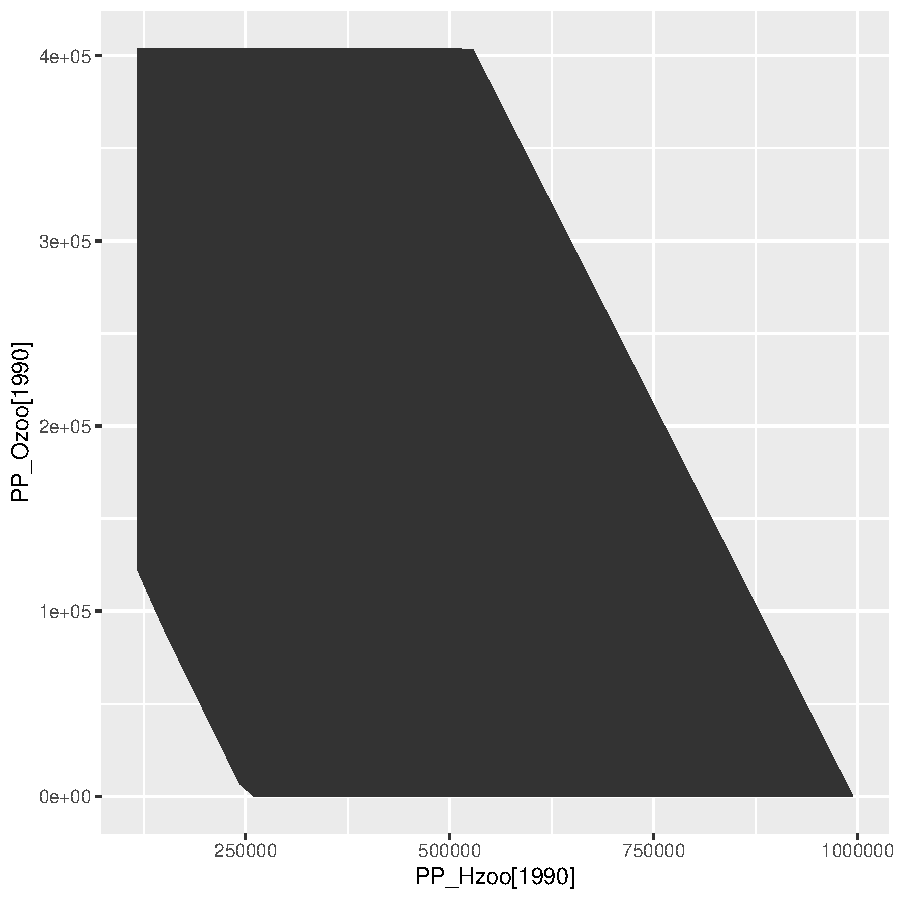
\includegraphics{barents_SM-011}

\clearpage

\section{Sampling polytope}

\subsection{Sampling}

\begin{Schunk}
\begin{Sinput}
> begin = Sys.time()
> SAMPLE <- sampleCaN(POLYTOPE, 
+                       N=100,thin=100, 
+                       nchain=2,
+                       ncore=2)
> end=Sys.time()
> end-begin
\end{Sinput}
\begin{Soutput}
Time difference of 13.5143 mins
\end{Soutput}
\end{Schunk}


\clearpage

\subsection{Convergence}

Using coda. 

\begin{Schunk}
\begin{Sinput}
> nchain(SAMPLE$mcmc)
\end{Sinput}
\begin{Soutput}
[1] 2
\end{Soutput}
\begin{Sinput}
> # summary(SAMPLE$mcmc)
\end{Sinput}
\end{Schunk}

Gelman diagnostics. Gelman and Rubin (1992) propose a general approach to monitoring convergence of MCMC output in which $ m > 1$ parallel chains are run with starting values that are overdispersed relative to the posterior distribution. Convergence is diagnosed when the chains have `forgotten' their initial values, and the output from all chains is indistinguishable. The gelman.diag diagnostic is applied to a single variable from the chain. It is based a comparison of within-chain and between-chain variances, and is similar to a classical analysis of variance.

\begin{Schunk}
\begin{Sinput}
> fluxY <- paste(FLUXES[2,1],'[1990]',sep="")
> gelman.diag(SAMPLE$mcmc[,fluxY])
\end{Sinput}
\begin{Soutput}
Potential scale reduction factors:

     Point est. Upper C.I.
[1,]       1.02       1.12
\end{Soutput}
\end{Schunk}


Autocorrelation function

\begin{Schunk}
\begin{Sinput}
> fluxZ <- paste(FLUXES[3,1],'[1990]',sep="")
> thinned_SAMPLE <- window(SAMPLE$mcmc,thin=2)
> thin(thinned_SAMPLE)
\end{Sinput}
\begin{Soutput}
[1] 2
\end{Soutput}
\begin{Sinput}
> acfplot(thinned_SAMPLE[,fluxZ])
\end{Sinput}
\end{Schunk}
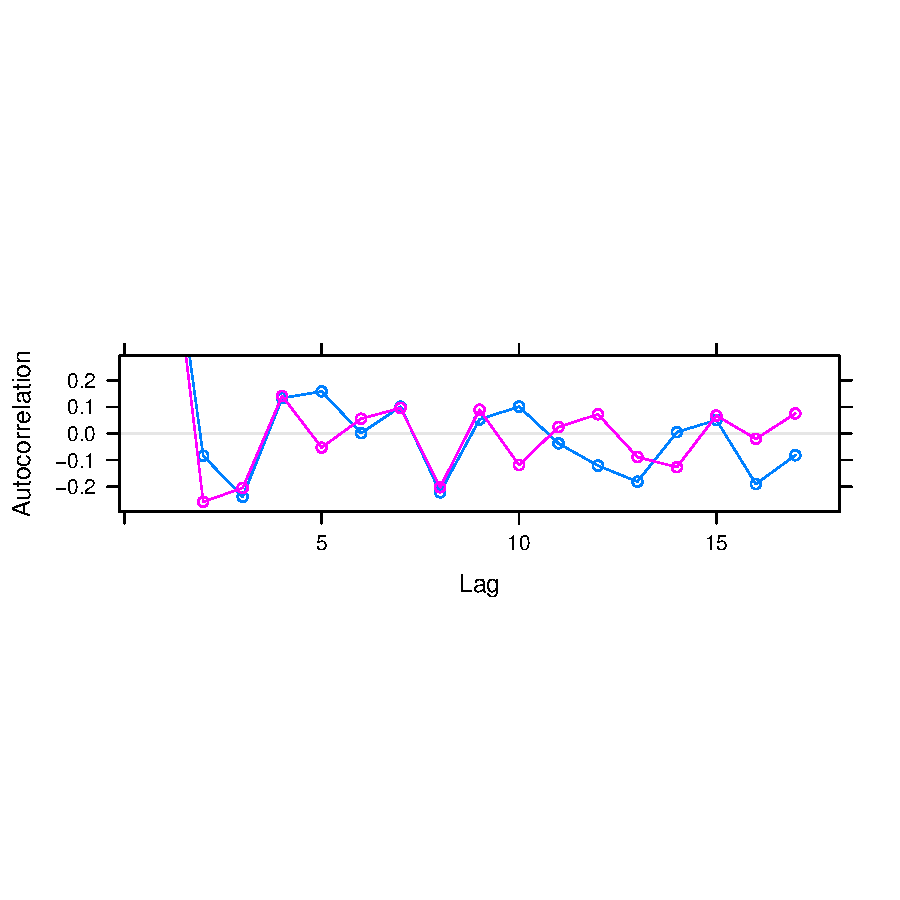
\includegraphics{barents_SM-015}

\clearpage

\subsection{Dynamics}

For several variables or flux, plots of sampled dynamics. 
\begin{Schunk}
\begin{Sinput}
> fluxX <- FLUXES[1,1]
> fluxY <- FLUXES[2,1]
> compA <- COMPONENTS[2,1] 
> compB <- COMPONENTS[3,1] 
> c(fluxX,fluxY,compA)
\end{Sinput}
\begin{Soutput}
[1] "PP_Hzoo" "PP_Ozoo" "Hzoo"   
\end{Soutput}
\end{Schunk}

\begin{Schunk}
\begin{Sinput}
> g <- ggSeries(SAMPLE, c(fluxX,fluxY,compA), TRUE)
> g + scale_y_log10() + guides(color = FALSE, fill = FALSE)
\end{Sinput}
\end{Schunk}
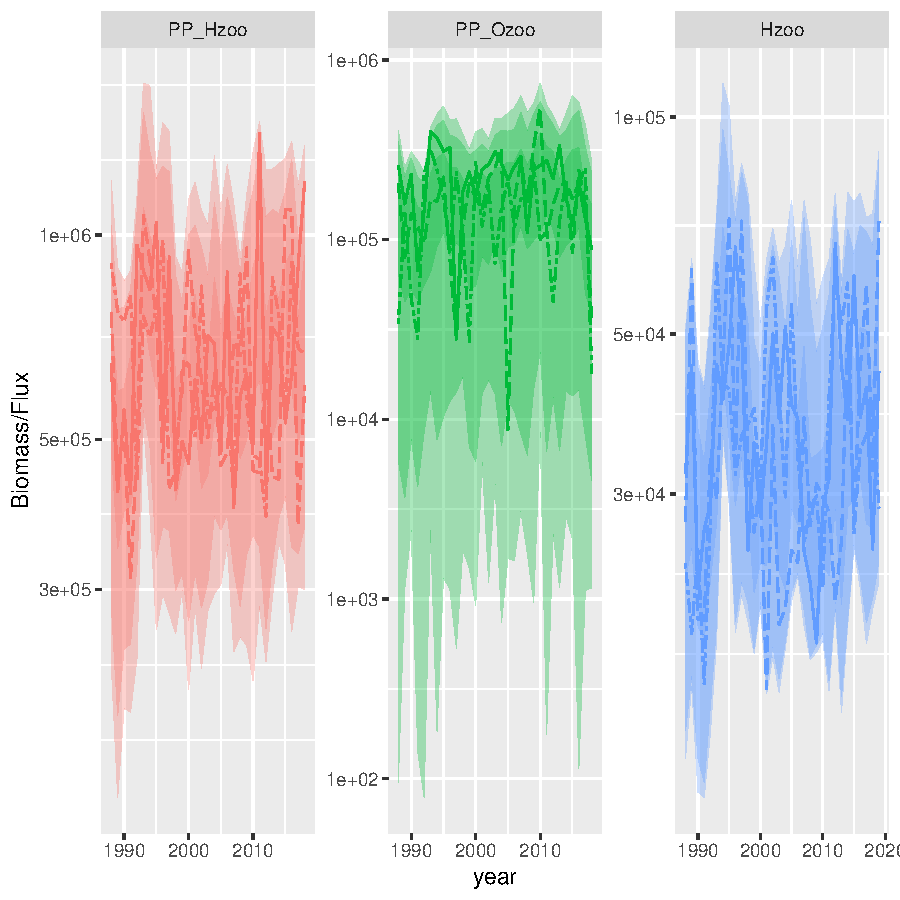
\includegraphics{barents_SM-017}

\clearpage

\subsection{Distribution}

For a component or a flux, for a year, the distribution of sampled values. 
\begin{Schunk}
\begin{Sinput}
> ggViolin(SAMPLE,c(fluxX,fluxY,compA),year=1990,TRUE)
\end{Sinput}
\end{Schunk}
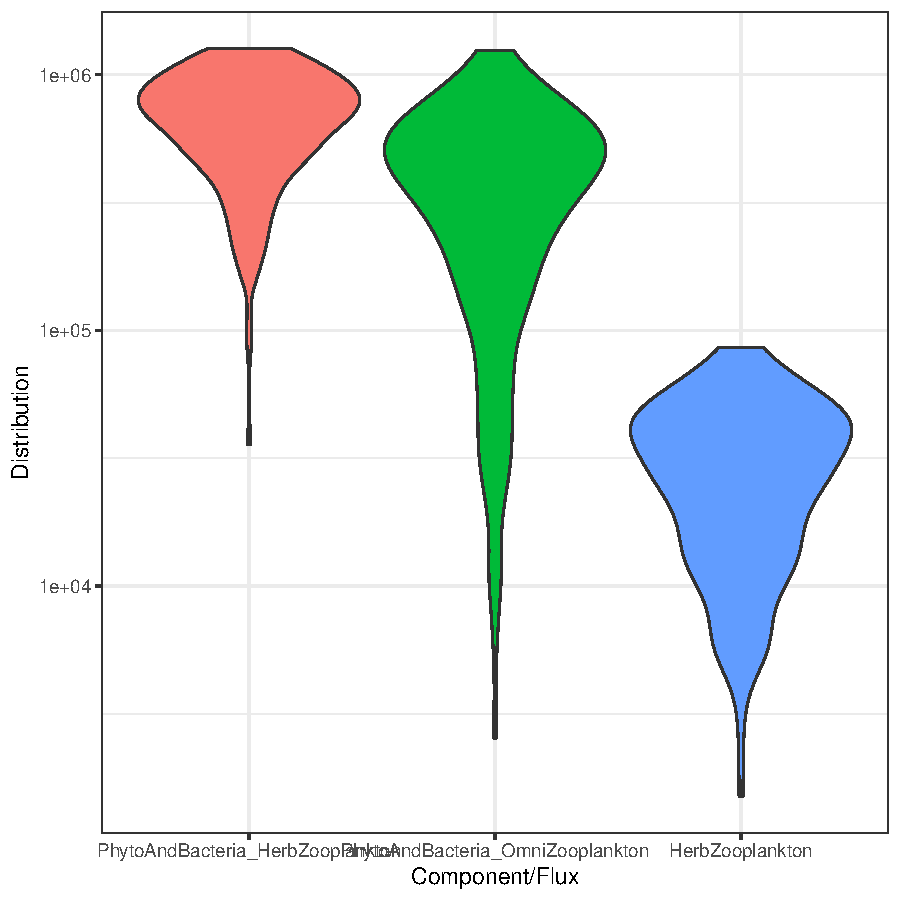
\includegraphics{barents_SM-018}


\clearpage

\subsection{Diet relationships}

\begin{Schunk}
\begin{Sinput}
> ggDiet(SAMPLE, compB)
\end{Sinput}
\end{Schunk}
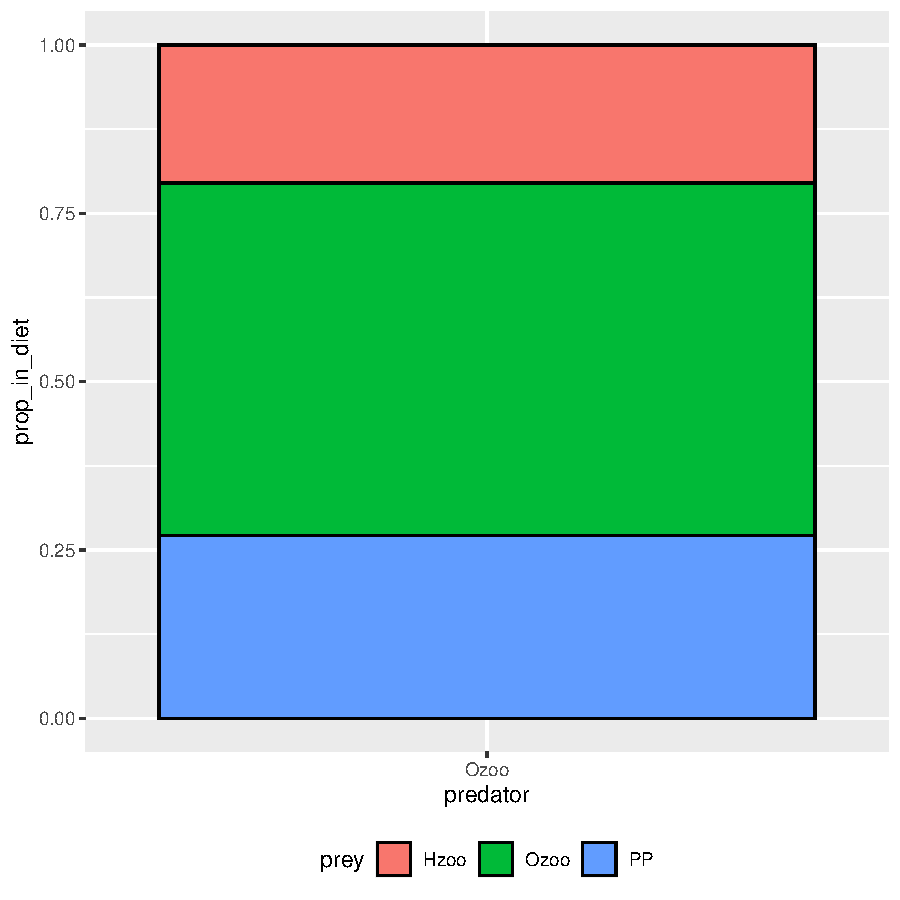
\includegraphics{barents_SM-019}

\subsection{Growth}

\begin{Schunk}
\begin{Sinput}
> ggGrowth(SAMPLE, compB)
\end{Sinput}
\end{Schunk}
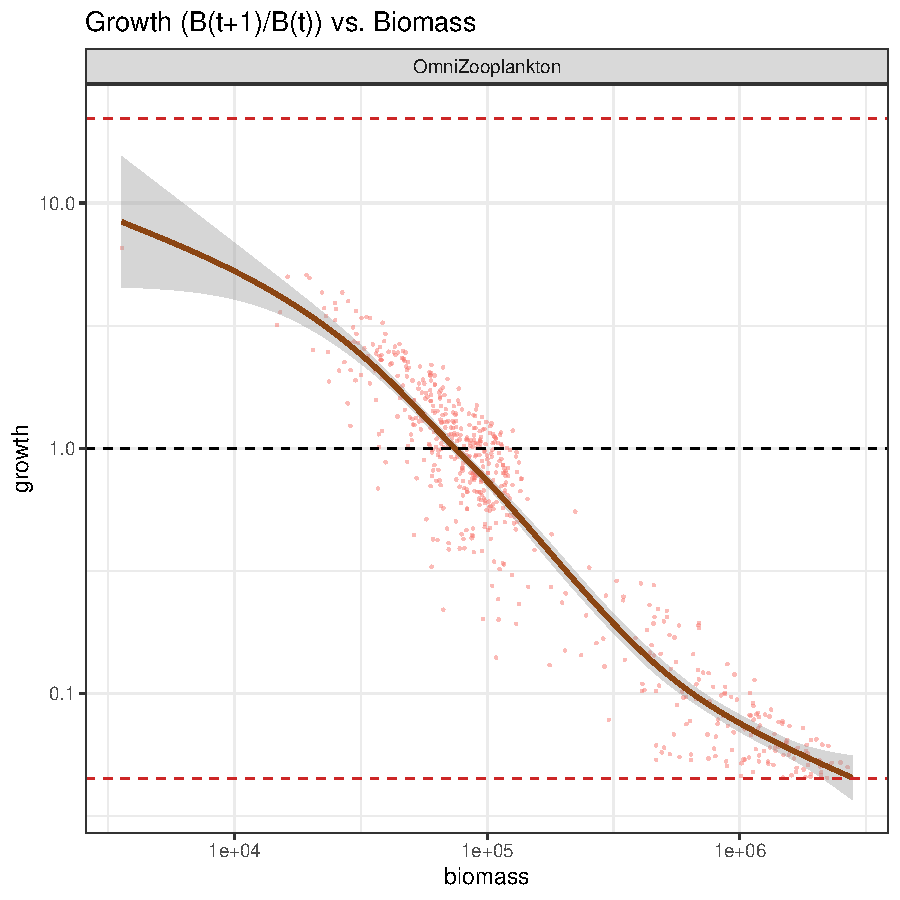
\includegraphics{barents_SM-020}

\subsection{Trophic relation}

\begin{Schunk}
\begin{Sinput}
> ggTrophicRelation(SAMPLE)
> # ggTrophicRelation(SAMPLE, compB)
\end{Sinput}
\end{Schunk}
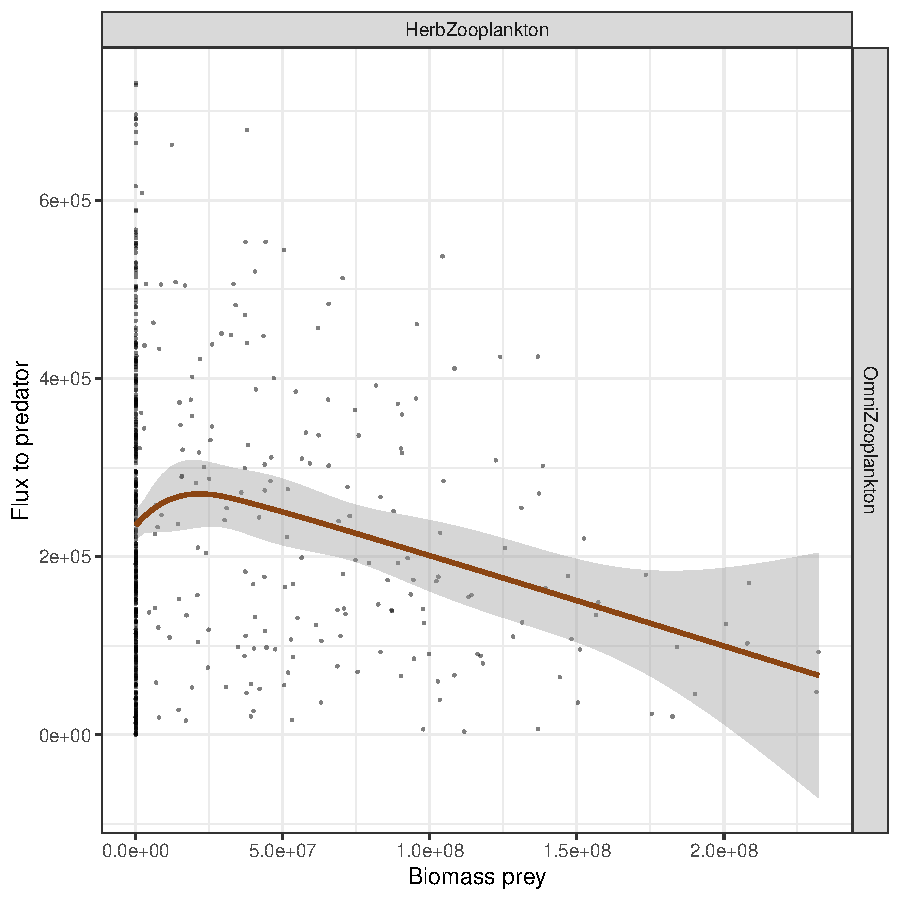
\includegraphics{barents_SM-021}

\subsection{Satiation}

\begin{Schunk}
\begin{Sinput}
> ggSatiation(SAMPLE, compB)
\end{Sinput}
\end{Schunk}
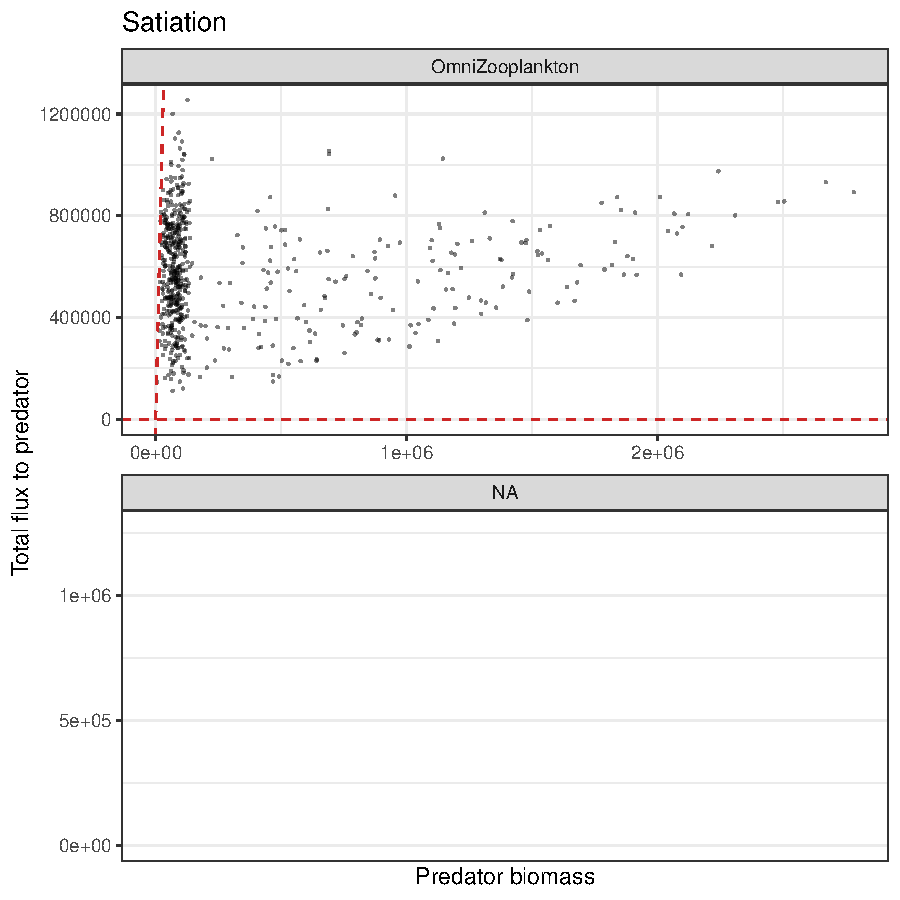
\includegraphics{barents_SM-022}

\section{Try and errors}

\subsection{Activating and desactivating constraint}

\begin{Schunk}
\begin{Sinput}
> # disactivate constraints C02
> constA = CONSTRAINTS[2,1]
> constA
\end{Sinput}
\begin{Soutput}
[1] "C02"
\end{Soutput}
\begin{Sinput}
> POLYTOPEA <- toggleConstraint(POLYTOPE, constA)
\end{Sinput}
\begin{Soutput}
 [1] "disactivate inequality C02 : 1998" "disactivate inequality C02 : 1999"
 [3] "disactivate inequality C02 : 2000" "disactivate inequality C02 : 2001"
 [5] "disactivate inequality C02 : 2002" "disactivate inequality C02 : 2003"
 [7] "disactivate inequality C02 : 2004" "disactivate inequality C02 : 2005"
 [9] "disactivate inequality C02 : 2006" "disactivate inequality C02 : 2007"
[11] "disactivate inequality C02 : 2008" "disactivate inequality C02 : 2009"
[13] "disactivate inequality C02 : 2010" "disactivate inequality C02 : 2011"
[15] "disactivate inequality C02 : 2012" "disactivate inequality C02 : 2013"
[17] "disactivate inequality C02 : 2014" "disactivate inequality C02 : 2015"
[19] "disactivate inequality C02 : 2016" "disactivate inequality C02 : 2017"
[21] "disactivate inequality C02 : 2018"
\end{Soutput}
\begin{Sinput}
> # disactivate constraints C02 for year 1991
\end{Sinput}
\end{Schunk}

\begin{Schunk}
\begin{Sinput}
> checkPolytopeStatus(POLYTOPEA)
\end{Sinput}
\begin{Soutput}
[1] "polytope ok"
\end{Soutput}
\end{Schunk}

\subsection{Building and analyzing sample}

\begin{Schunk}
\begin{Sinput}
> begin = Sys.time()
> SAMPLEA <- sampleCaN(POLYTOPEA, 
+                       N=100,thin=100, 
+                       nchain=2,
+                       ncore=2)
> end=Sys.time()
> end-begin
\end{Sinput}
\begin{Soutput}
Time difference of 14.12087 mins
\end{Soutput}
\end{Schunk}

\begin{Schunk}
\begin{Sinput}
> fluxX <- FLUXES[1,1]
> fluxY <- FLUXES[2,1]
> compA <- COMPONENTS[2,1] 
> compB <- COMPONENTS[3,1] 
> c(fluxX,fluxY,compA)
\end{Sinput}
\begin{Soutput}
[1] "PP_Hzoo" "PP_Ozoo" "Hzoo"   
\end{Soutput}
\begin{Sinput}
> g <- ggSeries(SAMPLEA, c(fluxX,fluxY,compA), TRUE)
> g + scale_y_log10() + guides(color = FALSE, fill = FALSE)
\end{Sinput}
\end{Schunk}
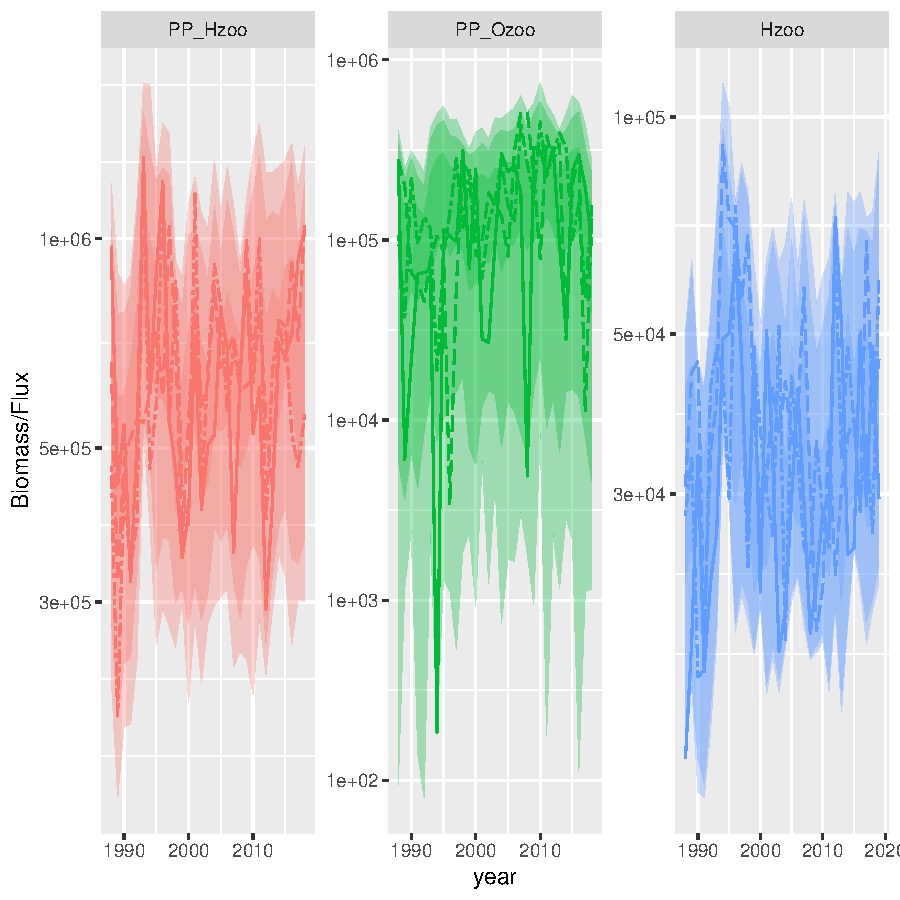
\includegraphics{barents_SM-026}

\end{document}
